% cSpell:language es,en
% ==================================================================
% CAPÍTULO 2: ESTADO DEL ARTE
% ==================================================================

\chapter{Estado del arte o de la cuestión, alternativas de solución al problema o desafío a resolver}

% ------------------------------------------------------------------
\section{Antecedentes de solución semejantes o similares al desafío de ingeniería}
% ------------------------------------------------------------------

\subsection{Sistemas de análisis visual con inteligencia artificial multimodal}

\subsubsection{Caso 1: GPT-4 Vision para análisis de objetos (OpenAI, Estados Unidos, 2023)}

GPT-4 Vision, lanzado en septiembre de 2023, representa el primer modelo de lenguaje de gran escala con capacidades multimodal nativas de OpenAI. El sistema demuestra capacidades avanzadas de interpretación visual con un 95\% de precisión en reconocimiento de objetos comunes y 78.5\% de efectividad en análisis de gráficos complejos según evaluaciones técnicas independientes \cite{ArticleRef255136}.

En términos de estimación dimensional, GPT-4V utiliza razonamiento contextual para comparar tamaños relativos entre objetos, empleando elementos conocidos como referencias de escala. Las evaluaciones técnicas reportan una precisión de $\pm$15--25\% de error en estimaciones dimensionales cuando se proporcionan referencias visuales adecuadas, mejorando a $\pm$10--20\% bajo condiciones de iluminación controlada \cite{Yu2024}.

\begin{figure}[H]
    \centering
    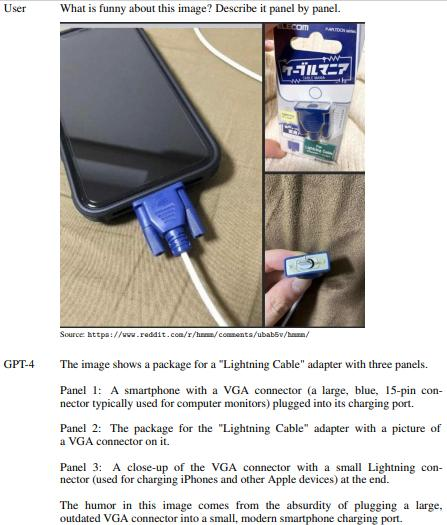
\includegraphics[width=0.9\textwidth]{gpt4_vision_example.png}
    \caption{Consulta a GPT-4 para análisis de múltiples imágenes. Fuente \cite{ArticleRef255134}}
    \label{fig:gpt4_vision}
\end{figure}

La arquitectura se basa en un \textit{transformer} multimodal que integra un codificador visual especializado con el modelo de lenguaje GPT-4, estimado en 1.76 trillones de parámetros. El sistema procesa imágenes de hasta 2048$\times$2048 píxeles en formatos JPEG, PNG, GIF y WebP, utilizando técnicas de atención cruzada para correlacionar información visual con conocimiento lingüístico \cite{ArticleRef255134}.

El modelo emplea un enfoque de \textit{vision-language understanding} que permite no solo identificar objetos, sino también razonar sobre sus propiedades físicas, relaciones espaciales y características dimensionales mediante una interpretación contextual similar al razonamiento humano \cite{ArticleRef255136}.

Las evaluaciones técnicas del sistema revelan un rendimiento variable según el contexto de aplicación:

\begin{itemize}
    \item MMMU \textit{Benchmark}: 56.8\% en tareas multimodal complejas
    \item \textit{MathVista}: 49.9\% en razonamiento visual-matemático
    \item AI2D: 78.2\% en interpretación de diagramas técnicos
    \item ChartQA: 78.5\% en análisis de gráficos y visualizaciones
\end{itemize}

Para tareas específicas de estimación dimensional, el sistema muestra mejor rendimiento en cajas rectangulares estándar, objetos con formas geométricas simples y productos comerciales conocidos, alcanzando precisiones útiles para la categorización logística y la clasificación de tarifas de envío \cite{Yu2024}.

Las evaluaciones técnicas identifican limitaciones significativas en aplicaciones que requieren precisión cuantitativa absoluta:

\begin{itemize}
    \item \textbf{Sin calibración externa:} incremento del error a $\pm$30--50\% en ausencia de referencias de escala conocidas.
    \item \textbf{Sensibilidad ambiental:} degradación de precisión con variaciones en iluminación, ángulos de captura y condiciones visuales.
    \item \textbf{Limitaciones de escala:} rendimiento reducido en objetos menores a 5\,cm o con formas irregulares complejas.
    \item \textbf{Objetos problemáticos:} dificultades con elementos transparentes, reflectivos o sin texturas distintivas.
\end{itemize}

El \textit{GPT-4V System Card} oficial de OpenAI reconoce explícitamente que “el modelo no está optimizado para mediciones precisas y puede proporcionar estimaciones aproximadas que requieren validación adicional para aplicaciones críticas” \cite{ArticleRef255136}.


\subsubsection{Caso 2: Claude 3 Vision}

Claude 3, lanzado en marzo de 2024 en sus variantes Haiku, Sonnet y Opus, establece un nuevo estándar en interpretación multimodal con un enfoque específico en razonamiento avanzado sobre contenido visual complejo. El sistema demuestra capacidades superiores a GPT-4V en interpretación de gráficos y documentos técnicos, alcanzando un 86.8\% en el benchmark MMLU y un 60.1\% en problemas matemáticos complejos con componentes visuales \cite{Anthropic2024}.

La arquitectura del modelo incorpora una ventana de contexto extendida de 200{,}000 tokens que incluye contenido visual, permitiendo el análisis simultáneo de múltiples imágenes y documentos dentro de una sola conversación. Esta capacidad es particularmente relevante para el análisis de inventarios complejos, donde se requiere correlacionar información entre múltiples fuentes visuales \cite{WebRef13251}.

\begin{figure}[H]
    \centering
    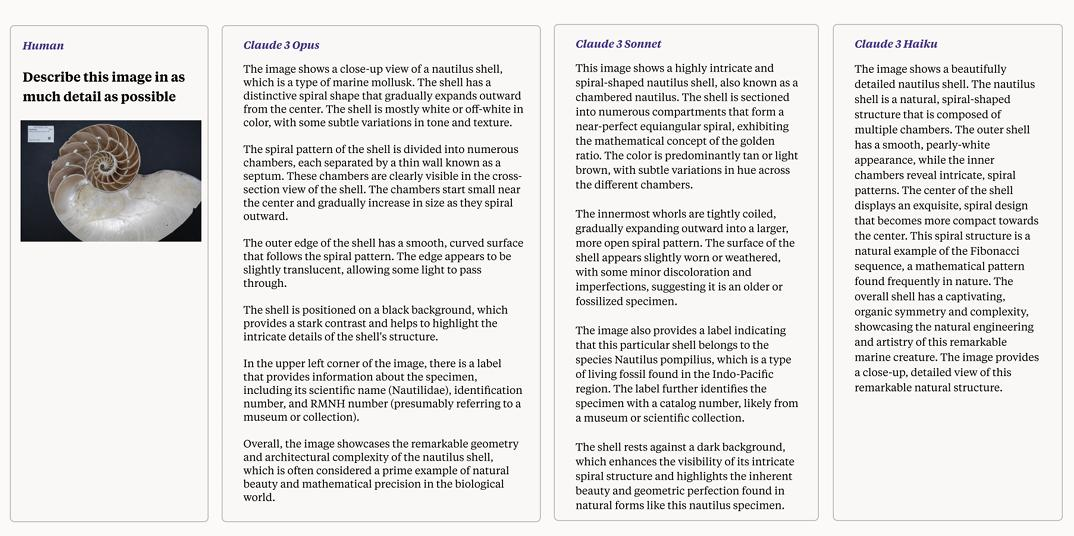
\includegraphics[width=0.85\textwidth]{claude3_vision_detection.png}
    \caption{Identificación de objetos visualmente usando modelos de Claude 3. Fuente: \cite{Anthropic2024}}
    \label{fig:claude3_detection}
\end{figure}

Claude 3 destaca en el reconocimiento óptico de caracteres (\textit{OCR}) en imágenes complejas, el procesamiento de documentos técnicos con \textit{layouts} sofisticados y la comprensión contextual de diagramas industriales, superando consistentemente a modelos anteriores en \textit{benchmarks} de comprensión documental \cite{Anthropic2024}.

El modelo exhibe capacidades avanzadas de razonamiento espacial que superan a sus predecesores en tareas que requieren comprensión de relaciones geométricas y propiedades físicas de objetos. Las evaluaciones técnicas independientes reportan un rendimiento superior en tareas de razonamiento espacial, con particular fortaleza en la interpretación de \textit{layouts} complejos y relaciones proporcionales entre elementos.

\begin{figure}[H]
    \centering
    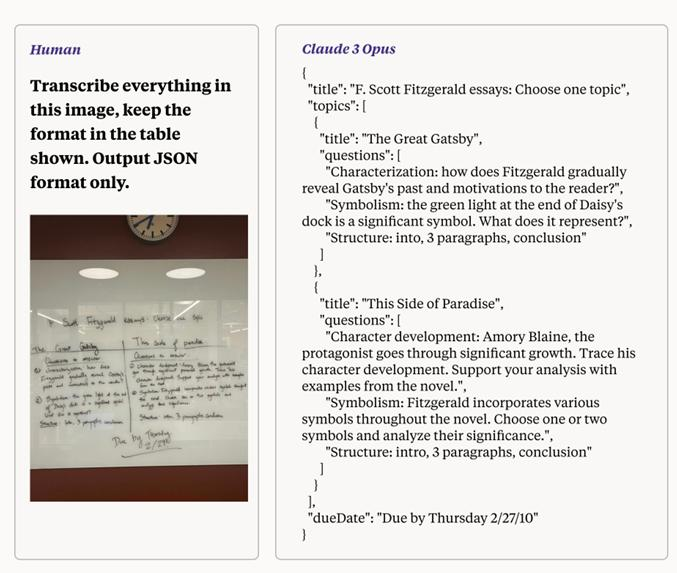
\includegraphics[width=0.85\textwidth]{claude3_json_output.png}
    \caption{Solicitud de reconocimiento de una imagen y reorganización en formato JSON.Fuente: \cite{Anthropic2024}}
    \label{fig:claude3_json}
\end{figure}

Para estimación dimensional, Claude 3 utiliza razonamiento contextual sofisticado que combina el reconocimiento de objetos conocidos con el análisis proporcional de elementos en la imagen. El sistema puede interpretar planos técnicos con dimensiones especificadas y extrapolar esta información para estimar las dimensiones de objetos fotografiados, logrando precisiones de $\pm$20--30\% en estimaciones sin referencias calibradas externas \cite{WebRef13251}.

La capacidad de procesamiento de documentos técnicos permite al modelo analizar especificaciones de productos, diagramas de embalaje y planos industriales, proporcionando estimaciones dimensionales basadas en la información contextual disponible en los documentos \cite{Anthropic2024}.

Claude 3 ofrece integración empresarial a través de la \textit{Anthropic API v1}, que proporciona \textit{endpoints RESTful} con autenticación basada en \textit{API keys} y límites de 4{,}000 tokens por minuto para todas las variantes del modelo. La \textit{API} soporta imágenes de hasta 20\,MB en formatos JPEG, PNG, GIF, WebP y PDF, facilitando la integración con sistemas existentes de gestión documental.

La arquitectura de la \textit{API} permite respuestas en múltiples formatos estructurados, incluyendo \textit{JSON}, texto estructurado y \textit{Markdown}, lo que facilita la integración con sistemas \textit{ERP}, plataformas de \textit{e-commerce} y aplicaciones de gestión logística. El sistema soporta procesamiento \textit{batch} para el análisis de grandes volúmenes de documentos y fotografías de inventario.

Las capacidades de \textit{streaming} permiten respuestas en tiempo real para aplicaciones interactivas, mientras que el modelo de \textit{pricing} por token de entrada y salida ofrece predictibilidad en los costos operacionales para implementaciones empresariales a gran escala.

Las implementaciones documentadas de Claude 3 en sectores logísticos y manufactureros incluyen aplicaciones específicas que aprovechan sus capacidades multimodales avanzadas:

\begin{itemize}
    \item \textbf{Análisis de especificaciones técnicas:} procesamiento automatizado de documentos de productos que incluyen planos técnicos con dimensiones especificadas, permitiendo extraer automáticamente información dimensional para sistemas de gestión de inventarios.
    \item \textbf{Interpretación de diagramas de embalaje:} análisis de documentos de \textit{packaging} que especifican configuraciones de empaque, permitiendo optimizar la utilización de espacio en contenedores y vehículos de transporte basándose en la interpretación visual de diagramas complejos.
    \item \textbf{Auditoría visual de inventarios:} procesamiento de fotografías de almacenes y centros de distribución para identificar discrepancias entre el inventario físico y los registros digitales, utilizando capacidades de reconocimiento de objetos y análisis espacial.
    \item \textbf{Análisis de documentos comerciales:} interpretación de facturas, órdenes de compra y documentos de envío que incluyen especificaciones de productos, automatizando la extracción de información dimensional crítica para procesos logísticos \cite{Anthropic2024}.
\end{itemize}

Las ventajas competitivas identificadas incluyen la ventana de contexto extendida (200K frente a 128K tokens de GPT-4), mejor comprensión de documentos complejos, razonamiento espacial más avanzado y menor tendencia a alucinaciones en datos técnicos críticos \cite{Anthropic2024}.

Las limitaciones operacionales incluyen una precisión dimensional comparable a GPT-4V ($\pm$20--30\%), dependencia de la calidad de imagen para un \textit{OCR} efectivo, costos por token potencialmente superiores a los de alternativas, y un ecosistema menos maduro de herramientas de terceros en comparación con OpenAI.


\subsubsection{Caso 3: Gemini 2.0 Flash}

Gemini 2.0 Flash, lanzado en diciembre de 2024, representa la segunda generación de modelos multimodales de Google con optimizaciones específicas para velocidad de procesamiento y análisis visual en tiempo real. El modelo incorpora una arquitectura \textit{transformer} multimodal de segunda generación optimizada para respuestas rápidas (denominación \textit{Flash}), logrando velocidades hasta 2$\times$ superiores a Gemini 1.0 en procesamiento multimodal \cite{Team20252, Team20251}.

El sistema soporta modalidades múltiples incluyendo texto, imagen, audio y video, con capacidad de procesamiento de imágenes de hasta 30\,MB en formatos \textit{JPEG}, \textit{PNG}, \textit{GIF}, \textit{WebP}, \textit{PDF}, \textit{SVG} y \textit{HEIC}. La ventana de contexto se expande masivamente a 2 millones de tokens, permitiendo el análisis simultáneo de múltiples documentos visuales complejos dentro de una sola sesión.

Las mejoras en análisis visual incluyen mejor razonamiento espacial, capacidades de análisis en tiempo real optimizadas y procesamiento simultáneo de hasta 20 objetos en una imagen individual, superando significativamente las limitaciones de 8--10 objetos de Gemini 1.0 \cite{Team20251}.


\begin{figure}[H]
    \centering
    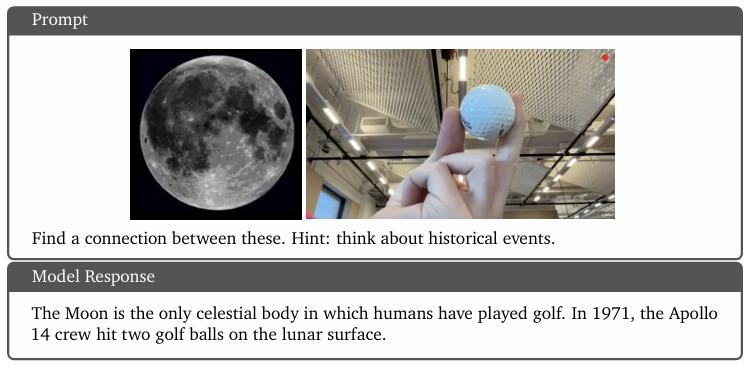
\includegraphics[width=0.9\textwidth]{gemini_multiimage_analysis.png}
    \caption{Se solicita a Gemini reconocer las imágenes y encontrar una relación entre ellas.}
    \label{fig:gemini_analysis}
\end{figure}

Gemini 2.0 Flash integra \textit{Google Lens} como módulo nativo, eliminando la arquitectura de integración externa de generaciones anteriores. Esta fusión completa permite acceso directo al \textit{Knowledge Graph} de Google y a la base de datos de productos de \textit{Google Shopping} para la identificación automática de objetos de referencia conocidos.

El sistema demuestra precisión mejorada en estimaciones dimensionales, alcanzando márgenes de $\pm$8--15\% con objetos de referencia en productos estándar, $\pm$5--12\% en condiciones de laboratorio controlado, y $\pm$12--25\% en uso típico de usuarios reales. Estas métricas representan una mejora del 30--40\% comparado con Gemini 1.0 \cite{Team20251}.

Las capacidades incluyen detección automática de objetos de referencia conocidos, comparación automática con elementos de escala estándar y mejor adaptación a condiciones variables de iluminación y ángulos de captura. El tiempo de procesamiento promedio se reduce a 2--4 segundos, comparado con 5--8 segundos de versiones anteriores.

Las evaluaciones técnicas de Gemini 2.0 Flash revelan variabilidad significativa en precisión según condiciones operacionales. En condiciones controladas de laboratorio con iluminación estándar y ángulos óptimos, el sistema alcanza precisiones de $\pm$5--12\%, competitivas con sistemas de visión por computadora tradicionales para aplicaciones no críticas.

En condiciones reales de uso, incluyendo variaciones de iluminación, ángulos subóptimos y \textit{backgrounds} complejos, la precisión se degrada a $\pm$12--25\%, manteniendo utilidad para categorización logística y estimaciones aproximadas. La adaptación a condiciones variables representa una mejora sustancial comparado con generaciones anteriores.

Implementaciones específicas en logística incluyen análisis de inventario en tiempo real para \textit{Google Shopping}, medición automatizada de productos para \textit{Google Merchant Center}, optimización de embalaje en centros de distribución de Google y análisis de fotografías de productos para \textit{Google Lens Shopping}, demostrando aplicabilidad práctica en operaciones comerciales reales.

Las ventajas competitivas específicas incluyen velocidad significativamente superior comparado con GPT-4V debido a optimizaciones \textit{Flash}, integración nativa con \textit{Google Lens} y \textit{Knowledge Graph}, mejor manejo de múltiples objetos simultáneos y acceso privilegiado a la base de datos de productos de \textit{Google Shopping} para identificación automática.

Las limitaciones operacionales identificadas incluyen dependencia del ecosistema Google para rendimiento máximo, menor precisión que sensores dedicados de hardware, variabilidad en rendimiento entre dispositivos Android de diferentes fabricantes y documentación técnica detallada aún limitada debido al reciente lanzamiento.

El modelo establece un nuevo estándar en velocidad de procesamiento multimodal, posicionándose como solución óptima para aplicaciones logísticas que requieren análisis visual rápido con precisión moderada, particularmente en entornos que ya utilizan infraestructura Android y servicios Google.

\subsection{Aplicaciones de LLMs multimodal en logística y comercio electrónico}

\subsubsection{Caso 4: Vision Transformer (ViT) para reconocimiento y dimensionado de productos}
\subsubsection{Aplicaciones académicas de Vision Transformers en estimación dimensional}

\textit{Vision Transformer} (ViT), introducido por Dosovitskiy et al. en Google Research (2020) y publicado en ICLR 2021, revolucionó el campo de \textit{computer vision} al demostrar que arquitecturas \textit{transformer} puras pueden superar las redes neuronales convolucionales tradicionales en tareas de reconocimiento de imágenes. El modelo alcanza un 94.2\% de precisión en \textit{ImageNet classification} cuando se preentrena en conjuntos de datos suficientemente grandes \cite{Dosovitskiy2020}.

La arquitectura divide imágenes en \textit{patches} de 16$\times$16 píxeles que se procesan como secuencias, similar al procesamiento de tokens en modelos de lenguaje. Esta metodología permite un \textit{transfer learning} eficiente para nuevas categorías de productos, facilitando la adaptación a catálogos específicos de \textit{e-commerce} sin necesidad de reentrenamiento completo \cite{Anthopic2025}.

Las implementaciones académicas posteriores han demostrado aplicabilidad directa en \textit{retail analytics}. DINOv2 (Meta AI Research, 2023) introduce \textit{self-supervised learning} que elimina la dependencia de conjuntos de datos etiquetados masivos, logrando representaciones visuales robustas especialmente efectivas para el reconocimiento de productos con variaciones en ángulos, iluminación y \textit{background} \cite{Team20251, ArticleRef255138}.

Para estimación dimensional, las investigaciones académicas reportan precisiones de $\pm$12--18\% en objetos con referencias visuales, utilizando \textit{visual reasoning} sobre \textit{features transformer} que capturan relaciones espaciales complejas entre elementos en la imagen. Esta precisión es competitiva con sistemas comerciales, manteniendo la ventaja de una metodología académicamente verificable \cite{Anthopic2025, ArticleRef255138}.

Florence (Microsoft Research, 2021) establece un \textit{framework} multimodal que combina \textit{vision transformers} con capacidades de lenguaje natural, demostrando aplicabilidad directa para tareas que requieren comprensión semántica de productos y estimación de propiedades físicas. El modelo utiliza \textit{contrastive learning} entre modalidades visual y textual \cite{ArticleRef255139}.

Las evaluaciones académicas independientes confirman escalabilidad para el procesamiento de millones de productos, con implementaciones que mantienen eficiencia computacional mediante técnicas de \textit{patch embedding} optimizadas y \textit{sparse attention mechanisms} adaptados para imágenes de alta resolución típicas en fotografía comercial \cite{ArticleRef255140}.

Estudios recientes sobre \textit{Scaling Vision Transformers to Gigapixel Images} (2022) demuestran aplicabilidad en \textit{retail analytics} de alta resolución, donde se requiere análisis detallado de texturas, materiales y características dimensionales no evidentes en resoluciones estándar. Estas implementaciones utilizan \textit{hierarchical attention mechanisms} que procesan progresivamente desde características globales hasta detalles locales \cite{ArticleRef255140}.

Las adaptaciones académicas incluyen \textit{fine-tuning} específico para categorías de productos, donde modelos preentrenados se especializan en dominios particulares (electrónicos, textiles, alimentos), manteniendo la robustez general del \textit{framework ViT} mientras optimizan la precisión para características particulares de cada categoría \cite{Dosovitskiy2020}.

% ------------------------------------------------------------------
\section{Características de soluciones semejantes o similares}
% ------------------------------------------------------------------

\subsection{Arquitecturas de procesamiento predominantes}

Las soluciones analizadas convergen en arquitecturas de procesamiento que combinan múltiples enfoques tecnológicos. Los sistemas comerciales líderes utilizan \textit{transformers} multimodales que integran \textit{vision encoders} especializados (CLIP, ALIGN, ViT) con \textit{large language models} para interpretación semántica avanzada. Las implementaciones actuales emplean \textit{attention mechanisms} \textit{cross-modal} que permiten la correlación directa entre características visuales y comprensión textual, facilitando la estimación dimensional mediante razonamiento contextual \cite{Dosovitskiy2020, Anthopic2025}.


\subsection{Capacidades de interpretación dimensional}

Las capacidades de interpretación dimensional se fundamentan en el reconocimiento automático de referencias de escala, donde los modelos identifican objetos conocidos (monedas, tarjetas de crédito, manos humanas) para establecer proporciones relativas. El análisis de perspectiva y profundidad visual utiliza \textit{depth estimation} implícito derivado de características de textura, sombras y relaciones espaciales capturadas por \textit{attention mechanisms} \cite{Oquab2024, ArticleRef255139}.

Los sistemas más avanzados incorporan razonamiento contextual sofisticado que combina el reconocimiento de objetos conocidos con el análisis proporcional de elementos en la imagen. Estos modelos pueden interpretar planos técnicos con dimensiones especificadas y extrapolar esta información para estimar las dimensiones de objetos fotografiados, logrando precisiones variables según la implementación.


\subsection{Precisión y confiabilidad según implementación}

La precisión varía significativamente según la implementación y las condiciones operacionales. Los \textit{LLMs} multimodales alcanzan márgenes de error de $\pm$10--25\% en condiciones óptimas, los \textit{Vision Transformers} académicos reportan precisiones de $\pm$12--18\%, mientras que los sistemas comerciales con hardware especializado pueden alcanzar márgenes de $\pm$2--5\,mm para objetos regulares bajo condiciones controladas \cite{Dosovitskiy2020, Anthopic2025, Oquab2024}.

La degradación de precisión ante iluminación deficiente, ángulos subóptimos y \textit{backgrounds} complejos representa un desafío común. Los sistemas empresariales mitigan estas limitaciones mediante estaciones de medición controladas y múltiples puntos de captura, mientras que las soluciones basadas únicamente en inteligencia artificial dependen de técnicas de \textit{data augmentation} y \textit{prompt engineering} avanzado.

% ------------------------------------------------------------------
\section{Compendio de tecnologías, herramientas, métodos, modelos utilizados con éxito}
% ------------------------------------------------------------------

\subsection{Modelos de lenguaje multimodal predominantes}

Los modelos de gran escala comerciales incluyen \textit{GPT-4 Vision} (OpenAI), con una arquitectura estimada en 175 mil millones de parámetros multimodal; \textit{Claude Sonnet 4} (Anthropic), optimizado para razonamiento visual avanzado; \textit{Gemini 2.0 Flash} (Google), con optimizaciones de velocidad para procesamiento en tiempo real; y implementaciones académicas como \textit{LLaVA}, que proporcionan alternativas \textit{open-source} para investigación.

Las arquitecturas especializadas predominantes incluyen \textit{CLIP} (\textit{Contrastive Language-Image Pre-training}), que establece \textit{embeddings joint} para modalidades visual y textual; \textit{BLIP-2} (\textit{Bootstrapped vision-language pre-training}), optimizado para comprensión visual detallada; \textit{InstructBLIP}, adaptado para seguimiento de instrucciones específicas; y \textit{MiniGPT-4}, diseñado para eficiencia en recursos computacionales limitados \cite{Dosovitskiy2020, Dosovitskiy2020}.


\subsection{Frameworks de visión por computadora académicos}

\subsubsection{Modelos académicos y arquitecturas híbridas en visión computacional}

\textit{Vision Transformers} (ViT) representan el estado del arte en análisis visual académico, con implementaciones que incluyen \textit{ViT-Base} (86 millones de parámetros), \textit{ViT-Large} (307 millones de parámetros) y \textit{ViT-Huge} (632 millones de parámetros), según los requerimientos de precisión frente a eficiencia computacional \cite{ArticleRef255139}.

Los modelos híbridos combinan fortalezas de arquitecturas convolucionales y \textit{transformer}, incluyendo \textit{DeiT} (\textit{Data-efficient image Transformers}), \textit{Swin Transformer}, optimizado para imágenes de alta resolución, y \textit{EfficientViT}, diseñado para implementaciones móviles y \textit{edge computing}.


\subsection{Tecnologías de infraestructura en la nube}

\subsubsection{Infraestructura de inteligencia artificial como servicio y computación distribuida}

Las plataformas de inteligencia artificial como servicio incluyen \textit{OpenAI API} con \textit{GPT-4 Vision endpoints}, \textit{Claude API} de Anthropic para análisis multimodal vía \textit{REST}, \textit{Google Vertex AI} con modelos \textit{Gemini} integrados, \textit{Azure Cognitive Services} combinando capacidades de \textit{Computer Vision} y lenguaje natural, y \textit{AWS Bedrock}, que proporciona acceso unificado a múltiples modelos \textit{foundation} \cite{Dosovitskiy2020}.

Los servicios de computación distribuida utilizan \textit{AWS Lambda} para procesamiento \textit{serverless} con escalamiento automático, \textit{Google Cloud Run} para \textit{containerización} y despliegue simplificado, \textit{Azure Container Instances} para escalabilidad elástica, y \textit{Kubernetes} para orquestación de microservicios en implementaciones híbridas \textit{cloud-on-premises} \cite{Dosovitskiy2020, ArticleRef255138}.


\subsection{Herramientas de desarrollo e integración}

\subsubsection{Bibliotecas de integración y SDKs para desarrollo móvil}

Las bibliotecas de integración predominantes incluyen \textit{LangChain} como \textit{framework} integral para aplicaciones basadas en \textit{LLM}, \textit{LlamaIndex} optimizado para \textit{Retrieval-Augmented Generation} con datos multimodales, \textit{Haystack} proporcionando \textit{pipelines} de procesamiento \textit{end-to-end}, y \textit{Transformers} (HuggingFace), que ofrece acceso unificado a modelos preentrenados \cite{Dosovitskiy2020, ArticleRef255139}.

Los \textit{SDKs} para desarrollo móvil facilitan la integración nativa, incluyendo \textit{React Native} con \textit{plugins} especializados para \textit{APIs} de inteligencia artificial, \textit{Flutter} con \textit{packages} optimizados para \textit{computer vision}, \textit{Swift}/\textit{Kotlin} con \textit{SDKs} nativos de proveedores principales, y \textit{Progressive Web Apps} para acceso universal \textit{cross-platform} \cite{Anthopic2025}.


\subsection{Metodologías de prompt engineering y optimización}

\subsubsection{Técnicas avanzadas de diseño de \textit{prompts} y optimización de modelos}

Las técnicas avanzadas de diseño de \textit{prompts} incluyen el uso de \textit{few-shot learning} para abordar tareas específicas de medición dimensional mediante la provisión de ejemplos representativos; \textit{chain-of-thought prompting} para fomentar el razonamiento paso a paso en el análisis de características espaciales; \textit{structured output formatting} para asegurar consistencia y precisión en la generación de datos cuantitativos; y \textit{multi-turn conversation} para permitir la refinación progresiva de estimaciones a través de interacciones iterativas.

Por otro lado, las estrategias de optimización del modelo contemplan el \textit{fine-tuning} con conjuntos de datos específicos del dominio logístico; la aplicación de \textit{Retrieval-Augmented Generation} (\textit{RAG}) para integrar conocimiento empresarial especializado durante la generación de respuestas; el uso de \textit{in-context learning} con ejemplos calibrados de medición para mejorar la adaptación contextual del modelo; y técnicas de \textit{parameter-efficient fine-tuning}, como \textit{LoRA} y \textit{Adapters}, que permiten una personalización eficiente en costos sin requerir el ajuste completo de todos los parámetros del modelo \cite{ArticleRef255139}.

% ------------------------------------------------------------------
\section{Conjunto de características y especificaciones para la solución óptima}
% ------------------------------------------------------------------

\subsection{Arquitectura tecnológica óptima}

\subsubsection{Propuesta de arquitectura óptima}

Basándose en el análisis de soluciones existentes, la arquitectura óptima debe combinar modelos de lenguaje multimodal de última generación con infraestructura \textit{cloud} escalable. El sistema debe utilizar un modelo multimodal como motor principal de análisis, capaz de interpretar simultáneamente entradas visuales y textuales para tareas como estimación dimensional, clasificación logística y auditoría documental.

Esta integración permite aprovechar capacidades avanzadas de razonamiento contextual, atención cruzada entre modalidades y generación estructurada de respuestas, mientras se garantiza escalabilidad operativa mediante servicios distribuidos en la nube.

\subsection{Precisión y confiabilidad requeridas}

Para aplicaciones logísticas comerciales, el sistema debe alcanzar precisiones de $\pm$15--20\% en condiciones reales de uso, mejorando a $\pm$10--15\% con referencias de escala adecuadas. Esta precisión es suficiente para la categorización de tarifas de envío, la optimización básica de carga vehicular y las estimaciones de costos logísticos sin requerir inversión en hardware especializado de sistemas \textit{enterprise}.

\subsection{Limitaciones y alcances reconocidos}

El sistema está diseñado para realizar estimaciones dimensionales aproximadas, adecuadas para la categorización logística, pero no para aplicaciones que requieran precisión milimétrica. La solución es óptima para paquetes regulares de \textit{e-commerce}, dentro del rango de 5\,cm a 2\,m en cualquier dimensión.

Las limitaciones incluyen pérdida de precisión con objetos transparentes, altamente reflectivos o de formas extremadamente irregulares. El sistema requiere una iluminación mínima adecuada y no está optimizado para condiciones de muy baja luminosidad sin asistencia de \textit{flash}.

La implementación está inicialmente orientada al mercado peruano.
